% \documentclass[pdfCover]{myreport} % 需要pdf封面
\documentclass{myreport}
\title{空间域的图像}
\author{陈伯硕}
\date{\today}

\def\MyProject{数字图像处理}

\fancyhead{} % Clear the headers
\renewcommand{\headrulewidth}{1pt} % Width of line at top of page
\fancyhead[L]{\MyProject}
\fancyhead[R]{\MyTitle} % Mark right [R] of page with Chapter name [\leftmark]


\usepackage{subfiles}
\begin{document}

\maketitle

\section{实验目的}

  \begin{enumerate}
    \item 熟悉python图像处理工具箱python-opencv。
    \item 了解计算图像的统计指标的方法及其在图像处理中的意义。
    \item 了解图像的几何操作,如改变图像大小、剪切、旋转等。
  \end{enumerate}

\section{实验内容}

  \subsection{读、写和显示图像文件}
    % \lstinputlisting[language=python]{../src/io.py}

    % \cref{fig:io}
    \begin{figure}[H]
      \centering
      \includegraphics[width = \textwidth]{io}
      \caption{图片来自必应2022-12-24封面图$(1080 \times 1920)$}
      \label{fig:io}
    \end{figure}

  \subsection{计算图像有关的统计参数}
    % \lstinputlisting[language=python]{../src/gray_describe.py}
    % \cref{t:}
    \begin{table}[H]
      \caption{图像有关的统计参数}
      \label{t:}
      \centering
      \begin{tabular}{cc}
      \toprule[1.5pt]
        count &  \num{2.073600e+06} \\
        mean  &  \num{1.246039e+02} \\
        std   &  \num{4.646401e+01} \\
        min   &  \num{0.000000e+00} \\
        25\%   & \num{ 9.000000e+01} \\
        50\%   & \num{ 1.230000e+02} \\
        75\%   & \num{ 1.650000e+02} \\
        max   &  \num{2.550000e+02} \\
        
        % \specialrule{0em}{8pt}{1pt}
      \bottomrule[1.5pt]
      \end{tabular}
    \end{table}
    
    % \cref{fig:kde}
    \begin{figure}[H]
      \centering
      \includegraphics[width = 0.6\textwidth]{kde}
      \caption{概率密度函数}
      \label{fig:kde}
    \end{figure}
  \subsection{操作的图像}
    \subsubsection{添加高斯噪声}
      % \cref{fig:noisy}
      \begin{figure}[H]
        \centering
        \includegraphics[width = 0.6\textwidth]{noisy}
        \caption{上图为原图,下图加入$\mu = 0, \sigma = 0.1$的高斯噪声}
        \label{fig:noisy}
      \end{figure}

      % \cref{t:}
      \begin{table}[H]
        \caption{统计结果对比}
        \centering
        \begin{tabular}{lcc}
        \toprule[1.5pt]
          {} &           raw &         noisy \\
          \midrule[1pt]
          count &  \num{2.073600e+06} &  \num{2.073600e+06} \\
          mean  &  \num{4.926115e-01} &  \num{4.928214e-01} \\
          std   &  \num{1.823940e-01} &  \num{2.069834e-01} \\
          min   &  \num{0.000000e+00} &  \num{0.000000e+00} \\
          25\%   & \num{ 3.554478e-01} &  \num{3.419813e-01} \\
          50\%   & \num{ 4.866933e-01} &  \num{4.939059e-01} \\
          75\%   & \num{ 6.523734e-01} &  \num{6.501337e-01} \\        \bottomrule[1.5pt]
          max    & 1                   & 1
        \end{tabular}
      \end{table}

      % \cref{fig:noisy_raw}
      \begin{figure}[H]
        \centering
        \includegraphics[width = 0.6\textwidth]{noisy_raw}
        \caption{与原图分布对比}
        \label{fig:noisy_raw}
      \end{figure}
    \subsubsection{改变图像大小}
      % \cref{fig:shrink}
      \begin{figure}[H]
        \centering
        \includegraphics[width = 0.6\textwidth]{shrink}
        \caption{skimage.transform.rescale(gray,0.25)将图片缩小为$70 \times 480$}
        \label{fig:shrink}
      \end{figure}
      % \cref{t:}
      \begin{table}[H]
        \caption{灰度图统计信息}
        \label{t:}
        \centering
        \begin{tabular}{ccc}
        \toprule[1.5pt]
          {} &           raw &        rotated \\
          \midrule[1pt]
            count &  \num{2.073600e+06} &  \num{129600.000000} \\
            mean  &  \num{4.926115e-01} &  \num{     0.492607} \\
            std   &  \num{1.823940e-01} &  \num{     0.166192} \\
            min   &  \num{0.000000e+00} &  \num{     0.030959} \\
            25\%   & \num{ 3.554478e-01} & \num{      0.374124} \\
            50\%   & \num{ 4.866933e-01} & \num{      0.487050} \\
            75\%   & \num{ 6.523734e-01} & \num{      0.633985} \\
            max   &  \num{1.000000e+00} &  \num{     0.915189} \\
          % \specialrule{0em}{8pt}{1pt}
        \bottomrule[1.5pt]
        \end{tabular}
      \end{table}
    \subsubsection{旋转图像}
      % \cref{fig:rotated}
      \begin{figure}[H]
        \centering
        \includegraphics[width = 0.6\textwidth]{rotated}
        \caption{skimage.transform.rotate 将图片旋转$30^\circ$}
        \label{fig:rotated}
      \end{figure}

      % \cref{fig:rotated_kde}
      \begin{figure}[H]
        \centering
        \includegraphics[width = 0.6\textwidth]{rotated_kde}
        \caption{统计指标对比}
        \label{fig:rotated_kde}
      \end{figure}
    \subsubsection{裁剪}
      % \cref{fig:clipped}
      \begin{figure}[H]
        \centering
        \includegraphics[width = 0.6\textwidth]{clipped}
        \caption{直接对矩阵操作进行裁剪}
        \label{fig:clipped}
      \end{figure}

      % \cref{fig:clipped_kde}
      \begin{figure}[H]
        \centering
        \includegraphics[width = 0.6\textwidth]{clipped_kde}
        \caption{裁剪后某些灰度值更集中}
        \label{fig:clipped_kde}
      \end{figure}
  \subsection{对图像空间域增强}
    \subsubsection{$\gamma$变换}
      % \cref{fig:gamma}
      \begin{figure}[H]
        \centering
        \includegraphics[width = 0.6\textwidth]{gamma}
        \caption{$\gamma = 0.5 <1$, $\gamma = 1$(原图), $\gamma = 2 > 1$}
        \label{fig:gamma}
      \end{figure}

      \begin{figure}[H]
        \centering
        \includegraphics[width = 0.6\textwidth]{gamma_gray}
        \caption{$\gamma = 0.5 <1$, $\gamma = 1$(灰度图), $\gamma = 2 > 1$}
        \label{fig:gamma}
      \end{figure}
      主观感觉灰度图的$gamma$变换对亮度的影响更大
    \subsubsection{均值滤波}
      % \cref{fig:avg}
      \begin{figure}[H]
        \centering
        \includegraphics[width = 0.6\textwidth]{avg}
        \caption{滤波核$N=1$(原图),滤波核$N=20$,滤波核$N=50$}
        \label{fig:avg}
      \end{figure}
    \subsubsection{图像锐化}
      % \cref{fig:fish}
      \begin{figure}[H]
        \centering
        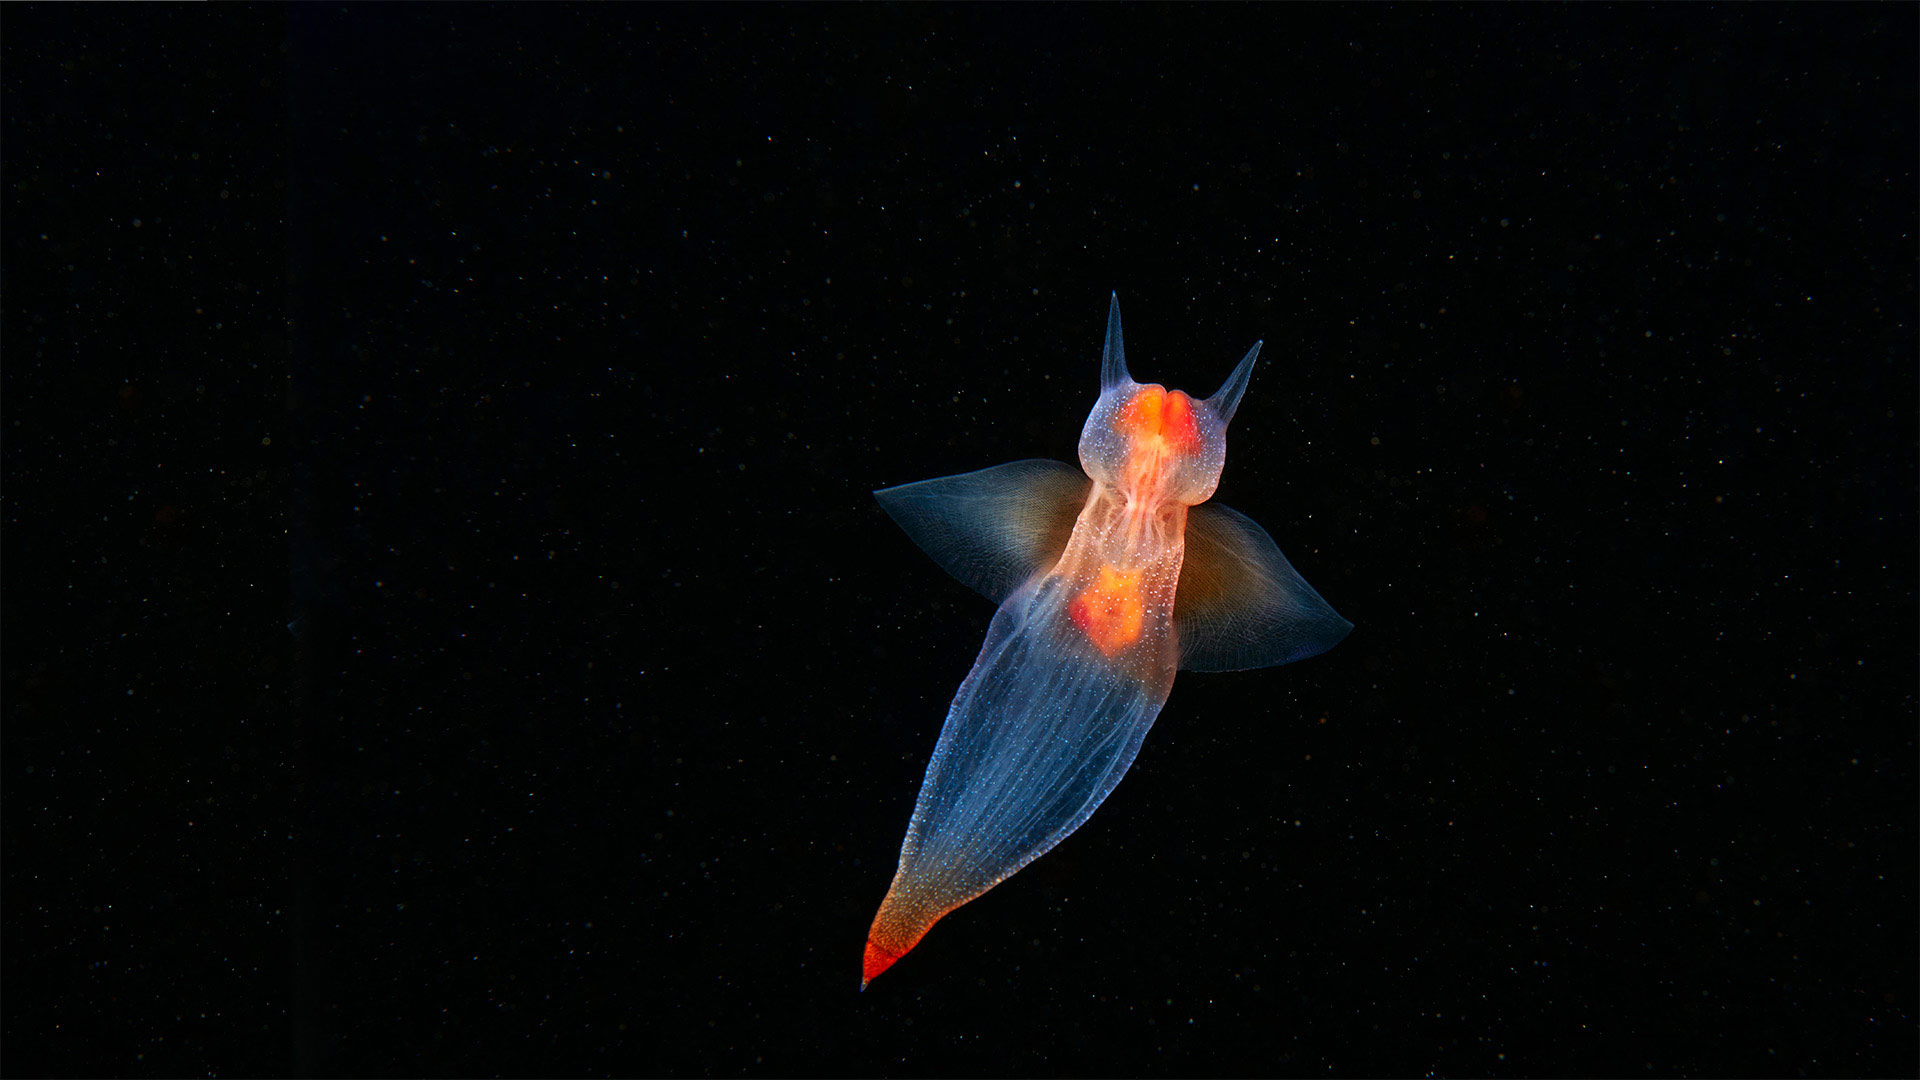
\includegraphics[width = 0.6\textwidth]{fish}
        \caption{图片来自 Bing 2022-10-29封面图}
        \label{fig:fish}
      \end{figure}

      \paragraph{Sobel}设$A$为原图像,则sobel滤波可表示为
      $$
        G_x = \begin{bmatrix}
            -1 & 0 & 1 \\
            -2 & 0 & 2 \\
            -1 & 0 & 1
        \end{bmatrix}
        \circledast A 
      $$
      
      $$
        G_y = \begin{bmatrix}
            1 & 2 & 1 \\
            0 & 0 & 0 \\
            -1 & -2 & -1
        \end{bmatrix}
        \circledast A 
      $$
      
      $$
        A'(x,y) = |G'_x(x,y)| + |G'_y(x,y)| 
      $$

      % \cref{fig:sobel}
      \begin{figure}[H]
        \centering
        \includegraphics[width = \textwidth]{sobel}
        \caption{依次为$G_x, G_y, A'$和skimagee.fiter.sobel的结果}
        \label{fig:sobel}
      \end{figure}

      \paragraph{滤波核2}
      $$
        G'_x = \begin{bmatrix}
            -1 & 0 & 1 \\
            -1 & 0 & 1 \\
            -1 & 0 & 1
        \end{bmatrix}
        \circledast A 
      $$
      
      $$
        G'_y = \begin{bmatrix}
            1 & 1 & 1 \\
            0 & 0 & 0 \\
            -1 & -1 & -1
        \end{bmatrix}
        \circledast A 
      $$
      
      $$
        A''(x,y) = |G'_x(x,y)| + |G'_y(x,y)| 
      $$

      % \cref{fig:sobel_compare}
      \begin{figure}[H]
        \centering
        \includegraphics[width = \textwidth]{sobel_vs_personal}
        \caption{$A',A''$结果对比}
        \label{fig:sobel_compare}
      \end{figure}
      两者整体上差别不大,Sobel算子的图灰度相差似乎更明显
      % \cref{fig:sobel_compare}
      \begin{figure}[H]
        \centering
        \includegraphics[width = 0.6\textwidth]{sobel_compare}
        \caption{两者的灰度分布}
        \label{fig:sobel_compare}
      \end{figure}
      \paragraph{自己设计一个$3 \times 3$ 的模板,
        能够检测$ \pm 45^\circ$倾斜方向的图像细节。}
        $$
          G_{13} = \begin{bmatrix}
              -1 & 0 & 1 \\
              -1 & 0 & 1 \\
              -1 & 0 & 1
          \end{bmatrix}
          \circledast A 
        $$
        
        $$
          G_{24} = \begin{bmatrix}
              1 & 1 & 1 \\
              0 & 0 & 0 \\
              -1 & -1 & -1
          \end{bmatrix}
          \circledast A 
        $$
        
        $$
          A_{1324}(x,y) = |G_{13}(x,y)| + |G_{24}(x,y)| 
        $$



        % \cref{fig:sharpen_13_24}
        \begin{figure}[H]
          \centering
          \includegraphics[width = \textwidth]{sharpen_13_24}
          \caption{$G_{13}, G_{24}$}
          \label{fig:sharpen_13_24}
        \end{figure}
        从鱼头部分可以看出$G_{13}$强调了$45^\circ$方向,
        鱼尾可以看出$G_{24}$强调了$-45^\circ$方向

        % \cref{fig:sharpen_13+24}
        \begin{figure}[H]
          \centering
          \includegraphics[width = 0.6\textwidth]{sharpen_13+24}
          \caption{最终效果}
          \label{fig:sharpen_13+24}
        \end{figure}
\section{心得和体会}
  本次实验接触图像处理的基本操作,
  本来先前使用opencv进行操作,
  不过在课上听同学说到了skimage这个库,
  接口更友好,文档更全面,
  并且选取的案例讲解图片非常明显,
  这些样例图片也很经典,
  利于学习,总体上看这个库体验更好,
  能与python 结合更加紧密,
  相比之下opencv的一些缩写不好理解,参数也比较混乱,
  代码阅读起含义容易忘记。

  比较不同库的效果的时候看文档能得到很多没有注意的细节.
  例如skimage说自己是RGB而opencv是BGR,
  所以opencv有些函数名不好记忆检索,
  或许与一开始的array构造有关,
  卷积操作scipy.ndimage.convolve 
  是skimage所使用的卷积操作,
  而cv2.filter2D用的是相连运算
  \footnote{\url{https://stackoverflow.com/questions/71275543/cv2-filter2d-vs-ndimage-convolve}},
  真正卷积的时候要把卷积核左右翻转,
  不过我们使用的时候卷积核有些不分左右,
  所以没有注意到这个细节,
  不过很有可能以后会犯错。


\begin{appendices} % 附录
  \includepdf[pages={1},pagecommand=\section*{源代码}]{attachment/build/image_processing.pdf}
  \includepdf[pages={2-},pagecommand=\section*{\quad}]{attachment/build/image_processing.pdf}

\end{appendices}
\end{document}
